\chapter{Fundamentalni Principi}

Stvarni problem knjige Živi Hram, prema desetom poglavlju Specijalnih Svjedočanstava je odstupanje od temelja naše vjere, koji je bio uspostavljen na početku našeg rada.

\egw{\textbf{Ovaj temelj je izgrađen od strane Najvećeg Radnika}, i \underline{održat će} se na oluji i buri. Hoće li mu se dopustiti da ovaj čovjek \textbf{predstavi doktrine koje opovrgavaju prošlo iskustvo} Božjeg naroda? Došlo je vrijeme za odlučnu akciju.}[SpTB02 54.2; 1904][https://egwwritings.org/read?panels=p417.276]

Kellogg je predstavio doktrine koje opovrgavaju prošlo iskustvo. Na drugom mjestu, ona je napisala o Kelloggu:

\egw{Silno sam zabrinuta za Dr. Kellogga. U mnogim aspektima, njegov put nije ugodan Gospodinu. Čini se da mu je \textbf{tako lako odstupiti od \underline{temeljnih principa}}. U velikoj je opasnosti da \textbf{prvotnu postojanost do kraja čvrsto ne održi}.}[Lt138-1902.5; 1902][https://egwwritings.org/read?panels=p9219.11]

Problem je bio u odstupanju od temeljnih principa—ali nisu svi to prepoznali. Posebice ključni i važni ljudi u radu; zaboravili su kako ih je Gospodin vodio i Njegovo učenje u prošlosti.

\egw{Nadala sam se da će doći do temeljite reformacije i da će se \textbf{principi} za koje smo se borili \textbf{u ranim danima} i koji su objavljeni u sili Duha Svetoga, \textbf{održavati}.}[SpTB02 56.3; 1904][https://egwwritings.org/read?panels=p417.287]

Koji su to bili principi za koje smo se borili u ranim danima? Što je to bio temelj naše vjere?

\egw{Kao narod moramo \textbf{čvrsto stajati na platformi vječne istine} koja je izdržala test i probu. Moramo se \textbf{držati sigurnih stupova naše vjere}. \textbf{\underline{Principi istine}} koje nam je Bog objavio \textbf{su naš jedini istiniti temelj}. Oni su nas učinili onim što jesmo...}[SpTB02 51.2; 1904][https://egwwritings.org/read?panels=p417.261]

\egwinline{Principi istine} koje nam je Bog objavio \egwinline{je naš jedini istiniti temelj}. Ona naziva te principe \textit{platformom vječne istine}. Ove principe ona naziva \egwinline{sigurnim stupovima naše vjere}[SpTB02 51.2; 1904][https://egwwritings.org/read?panels=p417.261].

Ona nas prisjeća naših prošlih iskustava pionira, poput Jamesa Whitea, Josepha Batesa, starješine Edsona, oca Piercea, kako je Bog radio na njima dok se \egwinline{točku po točku}, \egwinline{nisu sve \textbf{točke principa naše vjere} razbistrile}. Ona nas prisjeća kako je \egwinline{ovaj temelj izgrađen od strane Najvećeg Radnika,} i uvjerava nas da će se \egwinline{održati na oluji i buri}. U zaključku ona snažno potvrđuje volju Božju za nas u pogledu ovih principa. Bog nas \egwinline{poziva da se \textbf{držimo čvrstim zahvatom vjere, \underline{fundamentalnih principa} koji su zasnovani na neupitnom autoritetu}}.

Vidimo nekoliko različitih izraza koje je sestra White koristila za temelje naše vjere: “\textit{platforma vječne istine}”, “\textit{stupovi naše vjere}”, “\textit{principi istine}”, “\textit{točke principa}”, “\textit{međaši}”, “\textit{temeljni principi}”, i “\textit{fundamentalni principi}”. Ovi izrazi označavaju istu stvar—temelj naše vjere. Danas, kada čujemo te izraze, nekako nam ne daju nikakve konkretne informacije. Ali za adventiste sedmog dana u njeno vrijeme, ti principi označavali su vrlo određenu i jasnu stvar. Svi ovi pojmovi odnose se na javni sažetak vjere adventista sedmog dana pod nazivom \emcap{Fundamentalni Principi}, dodatno objašnjeno u nastavku.

Bog \egwinline{nas poziva da se \textbf{držimo čvrstim} zahvatom vjere, \textbf{\underline{fundamentalnih principa}} koji su \textbf{zasnovani na neupitnom autoritetu}.} Ovo se odnosi na glavne značajke adventističke vjere koje je Bog otkrio adventističkim pionirima \egwinline{nakon isteka vremena 1844,} kada je grupa oštroumnih, plemenitih i iskrenih ljudi \egwinline{tragala za istinom kao za skrivenim blagom.} To je bio \textit{temelj naše vjere}. Naši pioniri službeno su osnovali Crkvu Adventista Sedmog Dana 1863. godine i poučavali su te istine koje su nazivali “\textit{fundamentalni principi}.” No, adventisti sedmog dana često su bili pogrešno predstavljani u javnosti. Iz tog razloga, 1872. godine, naši pioniri objavili su dokument pod nazivom “\textit{Deklaracija Fundamentalnih Principa koje Uče i Prakticiraju Adventisti Sedmog Dana}” kako bi javno, ali ukratko, objavili koje \emcap{fundamentalne principe} adventisti sedmog dana uče i prakticiraju. Ovi \emcap{Fundamentalni Principi} redovito su se tiskali kao zasebna brošura, bili su prisutni u našim časopisima i godišnje su se tiskali u adventističkim godišnjacima tijekom života Ellen White.\footnote{Pogledajte Dodatak—\hyperref[appendix:timeline]{Fundamentalni Principi Vremenska crta} za više detalja.} Stoga, kada je Ellen White spominjala “\textit{fundamentalne principe}”, to nije bila nejasna ili neodređena izjava, jer je Crkva Adventista Sedmog Dana službeno i javno objavila što su ti \emcap{fundamentalni principi}. U predgovoru ovog dokumenta čitamo svrhu koja stoji iza njega.

\begin{figure}
    \centering
    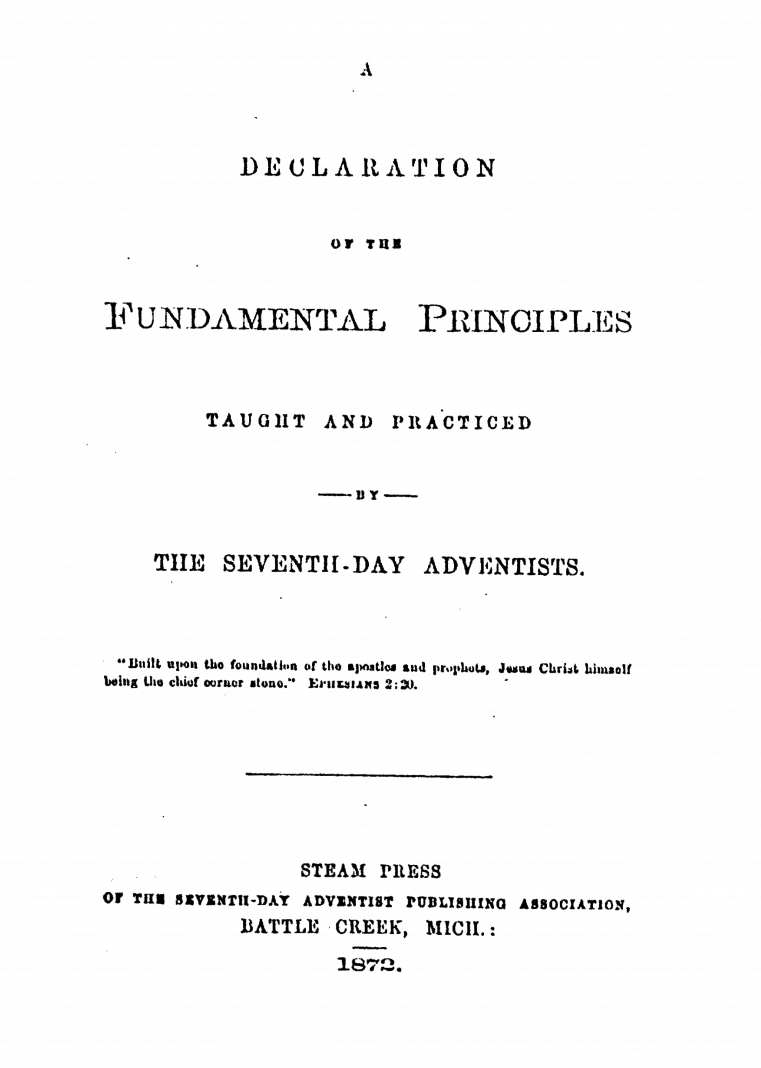
\includegraphics[width=1\linewidth]{images/declaration-of-the-fundamental-principles.PNG}
    \caption*{Sken Deklaracije Fundamentalnih Principa, 1872.}
    \label{fig:declaration-of-the-fundamental-principles}
\end{figure}

\others{U predstavljanju \textbf{javnosti} ovog \textbf{sinopsisa naše vjere}, želimo da bude jasno razumljivo da \textbf{nemamo nikakve članke vjere, kredo ili disciplinu }\textbf{\underline{izvan Biblije}}. \textbf{Ne} iznosimo ovo kao nešto što \textbf{ima ikakav autoritet nad našim narodom}, \textbf{niti je osmišljeno da osigura jednolikost među njima} \textbf{kao sustav vjerovanja}, \textbf{već je kratak iskaz \underline{onoga što jest i što je, sa velikom složnošću, vjerovano među njima}}. Često nam je potrebno odgovoriti na upite o ovoj temi, a ponekad i ispraviti lažne izjave koje se šire protiv nas, te ukloniti pogrešne dojmove koji su stvoreni kod onih koji nisu imali priliku upoznati se s našom vjerom i praksom. Naš jedini cilj je zadovoljiti tu potrebu.}

\othersnogap{\textbf{Kao adventisti sedmoga dana jednostavno želimo da se razumije naš stav}; i posebno smo zabrinuti za to jer postoje mnogi koji se nazivaju adventistima, a zastupaju gledišta s kojima ne možemo imati nikakve simpatije, od kojih su neka, smatramo, destruktivna za najjednostavnija i najvažnija načela izložena u Božjoj riječi...}[The Fundamental Principles 1872, p. 3.1][https://egwwritings.org/read?panels=p928.8]

Ovaj sinopsis vjere sastojao se od 25 točaka, koji su predstavljale \others{što jest i što je, sa velikom složnošću, vjerovano} od strane Adventista Sedmoga Dana. Ovih 25 točaka su sačinjavale \egwinline{\textbf{temelj} koji je bio \textbf{postavljen na početku} našeg rada \textbf{sa molitvom} i proučavanjem Riječi i Otkrivenja}. Sestra White je 1904 napisala da \egwinline{na \textbf{tom temelju} smo gradili \textbf{posljednjih pedeset godina}}. To su \egwinline{\textbf{fundamentalni principi koji su zasnovani na neupitnom autoritetu}}, na koje nas Bog \egwinline{poziva \textbf{da se držimo čvrstim} zahvatom vjere}. Drugim riječima, ponovila je, \egwinline{moramo se \textbf{držati sigurnih stupova naše vjere}}.

Godine 1904., sestra White je pisala o \egwinline{\textbf{naporima neprijatelja da potkopa temelje naše vjere}}. Pisala je o pokretu koji će \egwinline{sačinjavati \textbf{odstupanje} od doktrina koje stoje kao \textbf{stupovi naše vjere}}. Ova reformacija, ukoliko se prihvati, će odbaciti \egwinline{\textbf{principe istine} koje Bog u svojoj mudrosti dao crkvi ostatka} i \egwinline{\textbf{fundamentalni principi} koji su održavali posao posljednjih pedeset godina \textbf{bili bi proglašeni greškom}}. Ovaj pokret započeo je u vrijeme kada je Dr. John H. Kellogg izdao knjigu, “Živi Hram”.

\egw{U vremenu kada se izdala knjiga ‘Živi Hram’, u noćnoj viziji, \textbf{predstavljeni su mi prikazi koji su ukazivali na približavanje neke opasnosti}, te da se za nju moram pripremiti \textbf{pisanjem stvari} koje mi je Bog objavio \textbf{vezano za \underline{temeljne principe naše vjere}}.}[SpTB02 52.3; 1904][https://egwwritings.org/read?panels=p417.267]

Izdavanjem knjige “Živi Hram”, \textbf{fundamentalni principi naše vjere} \textbf{bili bi potkopani} \egwinline{kroz širenje \textbf{zavodljivih teorija}} koja ta knjiga sačinjava.

\egw{Bila sam upućena od strane Nebeskog glasnika da su neka rasuđivanja u knjizi ‘Živi Hram’ netočna i da će \textbf{ta razmišljanja odvesti u zabludu} umove onih koji nisu temeljito utemeljeni na \textbf{temeljnim principima} sadašnje istine. Ona uvode ono što je ništa više nego obična nagađanja \textbf{vezano za \underline{ličnost Boga i gdje je Njegova prisutnost}}.}[SpTB02 51.3; 1904][https://egwwritings.org/read?panels=p417.262]

Sestra White je poprilično precizno pokazala na koja razmišljanja u knjizi Živi Hram će \egwinline{\textbf{odvesti u zabludu}} od \egwinline{\textbf{temeljnih principa} sadašnje istine}. Ta razmišljanja su konkretno vezana za temu \egwinline{\textbf{ličnosti Boga i gdje je Njegova prisutnost}}.

Kao što smo ranije spomenuli, riječ ‘\textit{ličnost}’, u kontekstu devetnaestog stoljeća, je definirana kao “\textit{kvaliteta ili stanje koja nekog čine osobom}”\footnote{\href{https://www.merriam-webster.com/dictionary/personality}{Merriam-Webster Dictionary}, riječ ‘\textit{personality}’}. Drugim riječima, taj termin nam upućuje na odgovor na pitanje “\textit{što je to što nekoga čini osobom?}”. A što je to (kvaliteta ili stanje) što Boga čini osobom? To je pitanje koje se postavlja kada proučavamo temu o \emcap{ličnosti Boga}.

Razmišljanja dr. Kellogga po tim pitanjima, prikazana u knjizi Živi Hram, su \egwinline{netočna}. Sentimenti, \egwinline{\textbf{vezano za ličnost Boga i gdje je Njegova prisutnost}}, \egwinline{koji se zagovaraju u knjizi nisu nosili Božje odobrenje i da su oni zamka koju je neprijatelj pripremio za posljednje dane}. Pošto živimo u posljednjim danima, trebamo se zapitati vezano za ova pitanja. Također, valja nam i preispitati biblijsku opravdanost tvrdnji u \emcap{Fundamentalnim Principima} vezano za prisutnost i \emcap{ličnost Boga}. Kako Fundamentalni Principi definiraju Boga kao osobu, i što oni govore o Njegovoj prisutnosti?

Prva točka navedena ispod govori o \emcap{ličnosti Boga} i Njegovoj prisutnosti. Druga točka daje kontekst prvoj. Prije nego pročitate prve dvije točke Fundamentalnih Principa, zapitajte se nekoliko važnih pitanja: Tko se referira na pojam “jedan Bog”? Kako je Bog definiran kao osobom, odnosno koja je to kvaliteta ili stanje koje Ga čine osobom? Također, kako se objašnjava Božja prisutnost?

\others{“I – Da postoji \textbf{jedan Bog}, \textbf{\underline{osobno, duhovno biće}}, \textbf{stvoritelj svih stvari}, svemoguć, sveznajući i vječan, beskonačan u mudrosti, svetosti, pravdi, dobroti, istini i milosti; nepromjenjiv, i \textbf{\underline{svugdje prisutan po svom predstavniku, Svetome Duhu}}. Ps. 139:7.”}

\othersnogap{II – Da postoji \textbf{jedan Gospodin Isus Krist, }\textbf{\underline{Sin Vječnog Oca}}, onaj \textbf{\underline{po}}\textbf{ kojem je Bog stvorio sve stvari}, i po kojem sve postoji; …”}[Fundamentalni Principi 1889, točka br. 1., 2.,.] \footnote{Pogledajte \hyperref[chap:appendix]{Dodatak} za cijelu deklaraciju Fundamentalnih Principa.} \footnote{Od 1872. do 1914. Fundamentalni Principi ostali su stalni i nepromijenjeni, s iznimkom 1889. godine, kada je James Smith dodao tri nove točke. No tijekom svih tih godina, točke koje se odnose na \textit{prisutnost} i “\textit{ličnost Boga}” ostale su iste.}

U doba Ellen White, adventisti sedmoga dana vjerovali su u jednog Boga—osobno, duhovno biće, stvoritelja svih stvari—i vjerovali su da je taj Bog sve stvorio po Svojemu Sinu Isusu Kristu. Na Oca su upućivali kao na jednog Boga, dok su na Krista upućivali kao Božjeg Sina. Kvaliteta ili stanje koje Boga čini osobom izražena je pojmom “\textit{osobno, duhovno biće}”. Vezano za Njegovu prisutnost, \emcap{Fundamentalni Principi} tvrde kako je On svugdje prisutan preko svojega predstavnika, Duha Svetoga. Značenje ovih principa zahtijeva posebnu pažnju. Držeći se povijesnog konteksta, ovo će biti tema našeg daljnjeg proučavanja.

\section*{Test}

Najočitije, ovi \emcap{fundamentalni principi} ne sadrže doktrinu o Trojstvu! Preciznije, sentimenti “\textit{tri u jedan}” ili “\textit{jedan u tri}”, koji se odnose na Boga, nigdje se ne mogu pronaći—a koji su prisutni u današnjim \textit{Temeljnim Vjerovanjima}. Samo je Otac adresiran pod pojmom “\textit{jedan Bog}”. No prije nego požurite sa brzim zaključcima i osudite doktrinu o Trojstvu kao\egwinline{\textbf{zavodljive teorije}} koje\egwinline{\textbf{potkopavaju temelje naše vjere}}, molimo vas imajte na umu da sestra White predočava detaljnu listu karakteristika koje se moraju ispuniti kako bi se doktrina nazvala takvom.

Ukoliko se doktrina o Trojstvu postavlja pod pitanje, tada trinitarijanski sentimenti moraju:
\begin{itemize}
    \item lišiti Božji narod njihovog prošlog iskustva
    \item uništiti \emcap{ličnost Boga}
    \item srušiti stupove naše vjere ili odvesti od naših prvobitnih temeljnih principa
    \item biti prikazani kao da ih Ellen White podupire
\end{itemize}

Nije nam namjera baviti se nijednom Kelloggovom zavodljivom teorijom, već radije proučavati \emcap{ličnost Boga} u njezinoj povijesnoj pozadini. Dok to činimo, suočit ćemo se s dokazima sestre White koja reaktivno upozorava crkvu na navedene karakteristike.

% Fundamentalni Principi

\begin{titledpoem}
    \stanza{
        Najveći Radnik temelj je izgradio, \\
        Božjem narodu put je pripremio. \\
        Istine kroz molitvu otkrivene, \\
        Na neupitnom autoritetu utemeljene.
    }

    \stanza{
        Bog kao jedno osobno, duhovno biće, \\
        Po Duhu prisutan, svemoćno, sveznajuće. \\
        Krist kao Sin Vječnoga Oca stoji, \\
        Ove stupove vjere čvrsto drži i ne boji.
    }

    \stanza{
        Kad ljudi od principa ovih odstupe, \\
        Novim učenjima temelje potkopaju, \\
        Mudrost vjekova brzo odbacuju, \\
        I Božji put otkriven tužno narušavaju.
    }

    \stanza{
        Drži čvrsto istinu nepokolebljivim stiskom, \\
        Ne daj da vjera od sidra sklizne niskom. \\
        Jer što je Bog kroz pionire uspostavio, \\
        Kroz oluju i buru vječno je utvrdio.
    }
\end{titledpoem}